% SF1A: Illustration of the computational mechanism and the 4 directions of target sequence
% 

\documentclass[tikz, border=2pt]{standalone}
\usepackage{helvet}
\usepackage{amsmath}
\renewcommand{\familydefault}{\sfdefault}
\usetikzlibrary{decorations.pathreplacing, arrows.meta, positioning, calc}

\begin{document}
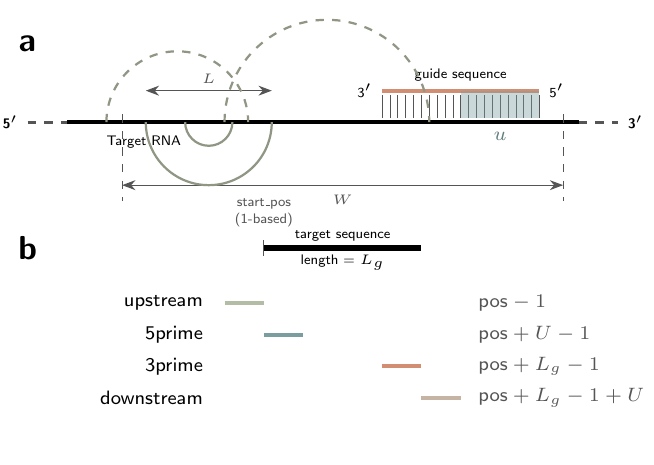
\begin{tikzpicture}[
    x=1cm, y=1cm,
    font=\sffamily,
    >=Stealth
]
    % 强制锁定画布尺寸：7.6cm x 5.2cm (约 3 x 2 英寸)
    \path[use as bounding box] (0, 1.2) rectangle (7.6, -4.0);

    % ==========================================
    % 定义淡雅配色系 (与 R 语言主图完全统一)
    % ==========================================
    \definecolor{mute3p}{HTML}{D28E72}    % 3prime: 淡砖红
    \definecolor{mute5p}{HTML}{7A9E9F}    % 5prime: 灰蓝色
    \definecolor{muteup}{HTML}{B3BCA4}    % upstream: 鼠尾草绿
    \definecolor{mutedn}{HTML}{C5B4A3}    % downstream: 暖灰
    \definecolor{darkgray}{HTML}{555555}  % 辅助线/文字灰

    % ==========================================
    % Panel a: 运算机制 (W, L, u)
    % ==========================================
    \node[font=\large\bfseries] at (0, 1.0) {a};

    % 1. Target RNA Backbone
    \draw[dashed, line width=1.2pt, darkgray] (0, 0) -- (0.5, 0);
    \draw[line width=1.5pt] (0.5, 0) -- (7.0, 0) node[pos=0.15, below=1pt, font=\tiny] {Target RNA};
    \draw[dashed, line width=1.2pt, darkgray] (7.0, 0) -- (7.5, 0);
    
    \node[left, font=\tiny\bfseries] at (0, 0) {5$'$};
    \node[right, font=\tiny\bfseries] at (7.5, 0) {3$'$};

    % 2. 局部折叠窗口 W (虚线与箭头)
    \draw[dashed, darkgray] (1.2, 0.1) -- (1.2, -1.0);
    \draw[dashed, darkgray] (6.8, 0.1) -- (6.8, -1.0);
    \draw[<->, darkgray] (1.2, -0.8) -- (6.8, -0.8) node[midway, below, font=\tiny] {$W$};

    % 3. 最大配对距离 L (箭头)
    \draw[<->, darkgray] (1.5, 0.4) -- (3.1, 0.4) node[midway, above=-1pt, font=\tiny] {$L$};

    % 4. Guide Sequence 与碱基配对
    % Guide 线 (3' 到 5')
    \draw[line width=1.5pt, mute3p] (4.5, 0.4) -- (6.5, 0.4);
    \node[above, font=\tiny] at (5.5, 0.4) {guide sequence};
    \node[left, font=\tiny] at (4.5, 0.4) {3$'$};
    \node[right, font=\tiny] at (6.5, 0.4) {5$'$};

    % 碱基配对 (细灰线密集排列)
    \foreach \i in {0,1,...,20} {
        \draw[very thin, darkgray] (4.5 + \i*0.1, 0.05) -- (4.5 + \i*0.1, 0.35);
    }

    % u 区域 (5prime 的开放特征区)
    \fill[mute5p, opacity=0.4] (5.5, 0.05) rectangle (6.5, 0.4);
    \node[below, font=\scriptsize, text=mute5p!80!black] at (6.0, 0.0) {$u$};

    % 5. 绿色弧线：表示允许与禁止的配对
    % 允许的配对 (实线，距离 <= L)
    \draw[muteup!80!black, thick] (1.5, 0) arc (180:360:0.8);
    \draw[muteup!80!black, thick] (2.0, 0) arc (180:360:0.3);
    % 禁止的配对 (虚线，距离 > L 或超出 W)
    \draw[muteup!80!black, thick, dashed] (1.0, 0) arc (180:0:0.9);
    \draw[muteup!80!black, thick, dashed] (2.5, 0) arc (180:0:1.3);


    % ==========================================
    % Panel b: Target Sequence & 4 Directions 代码映射
    % ==========================================
    \node[font=\large\bfseries] at (0, -1.6) {b};

    % Target sequence (黑色粗实线, 代表 L_g 区域)
    \draw[line width=2pt] (3.0, -1.6) -- (5.0, -1.6);
    \node[above=-1pt, font=\tiny] at (4.0, -1.6) {target sequence};
    \node[below=-1pt, font=\tiny] at (4.0, -1.6) {length = $L_g$};

    % start_pos 标注 (精准对齐在 target 左边缘)
    \draw[darkgray, thin] (3.0, -1.5) -- (3.0, -1.7);
    \node[above, font=\tiny, align=center, text=darkgray] at (3.0, -1.45) {start\_pos\\(1-based)};

    % 定义高度变量
    \def\yup{-2.3}
    \def\yfiv{-2.7}
    \def\ythr{-3.1}
    \def\ydwn{-3.5}
    \def\txtL{2.35} % 左侧定义文字的 X 坐标
    \def\txtR{5.6}  % 右侧代码文字的 X 坐标

    % 1. upstream (定位在 target 前1位)
    \node[left, font=\scriptsize] at (\txtL, \yup) {upstream};
    \draw[line width=1.5pt, muteup] (2.5, \yup) -- (3.0, \yup);
    \node[right, font=\scriptsize, text=darkgray] at (\txtR, \yup) {$\text{pos} - 1$};

    % 2. 5prime (定位在 target 内部长度 U 的区间)
    \node[left, font=\scriptsize] at (\txtL, \yfiv) {5prime};
    \draw[line width=1.5pt, mute5p] (3.0, \yfiv) -- (3.5, \yfiv);
    \node[right, font=\scriptsize, text=darkgray] at (\txtR, \yfiv) {$\text{pos} + U - 1$};

    % 3. 3prime (定位在 target 最末端)
    \node[left, font=\scriptsize] at (\txtL, \ythr) {3prime};
    \draw[line width=1.5pt, mute3p] (4.5, \ythr) -- (5.0, \ythr);
    \node[right, font=\scriptsize, text=darkgray] at (\txtR, \ythr) {$\text{pos} + L_g - 1$};

    % 4. downstream (定位在 target 末端之后长度 U 的区间)
    \node[left, font=\scriptsize] at (\txtL, \ydwn) {downstream};
    \draw[line width=1.5pt, mutedn] (5.0, \ydwn) -- (5.5, \ydwn);
    \node[right, font=\scriptsize, text=darkgray] at (\txtR, \ydwn) {$\text{pos} + L_g - 1 + U$};

\end{tikzpicture}
\end{document}